\documentclass[convert={density=72,outext=.png}]{standalone}
\usepackage{tikz}
\usetikzlibrary{shapes.geometric, arrows}
\usepackage{amsmath}

\tikzstyle{node} = [rectangle, text centered, align=center, fill=white]
\tikzstyle{stealthnode} = [rectangle, text centered, align=center, color=gray,
                           fill=white]
\tikzstyle{arrow} = [thick,>=stealth]
\tikzstyle{stealtharrow} = [thick,>=stealth, color=gray, dashed]

\tikzstyle{back1} = [xshift=0.8cm, yshift=1.2cm]
\tikzstyle{back2} = [xshift=1.6cm, yshift=2.4cm]
\tikzstyle{back3} = [xshift=2.4cm, yshift=3.6cm]
\tikzstyle{front1} = [xshift=-1.2cm, yshift=-1.8cm]

\newcommand{\drawLinewithBG}[3]
{
    \draw [white,line width=7pt, opacity=1.0]  (#1) -- (#2);
    \draw [#3] (#1) -- (#2);
}

\newcommand{\drawIntersectLine}[5]
{
    \draw [#4!50,line width=7pt, opacity=0.5]  (#1) -- (#2);
    \draw [#3, color = #5] (#1) -- (#2);
}

\newcommand{\drawFace}[4]
{
  \fill [color=#4!50, opacity = 0.5] (#1) -- (#2) -- (#3) -- (#1);
  \begin{scope}
  \draw [color=white, line width=7pt, opacity=1.0] (#1) -- (#2) -- (#3) -- (#1);
  \end{scope}
  \draw (#1) -- (#2) -- (#3) -- (#1);
}

\begin{document}

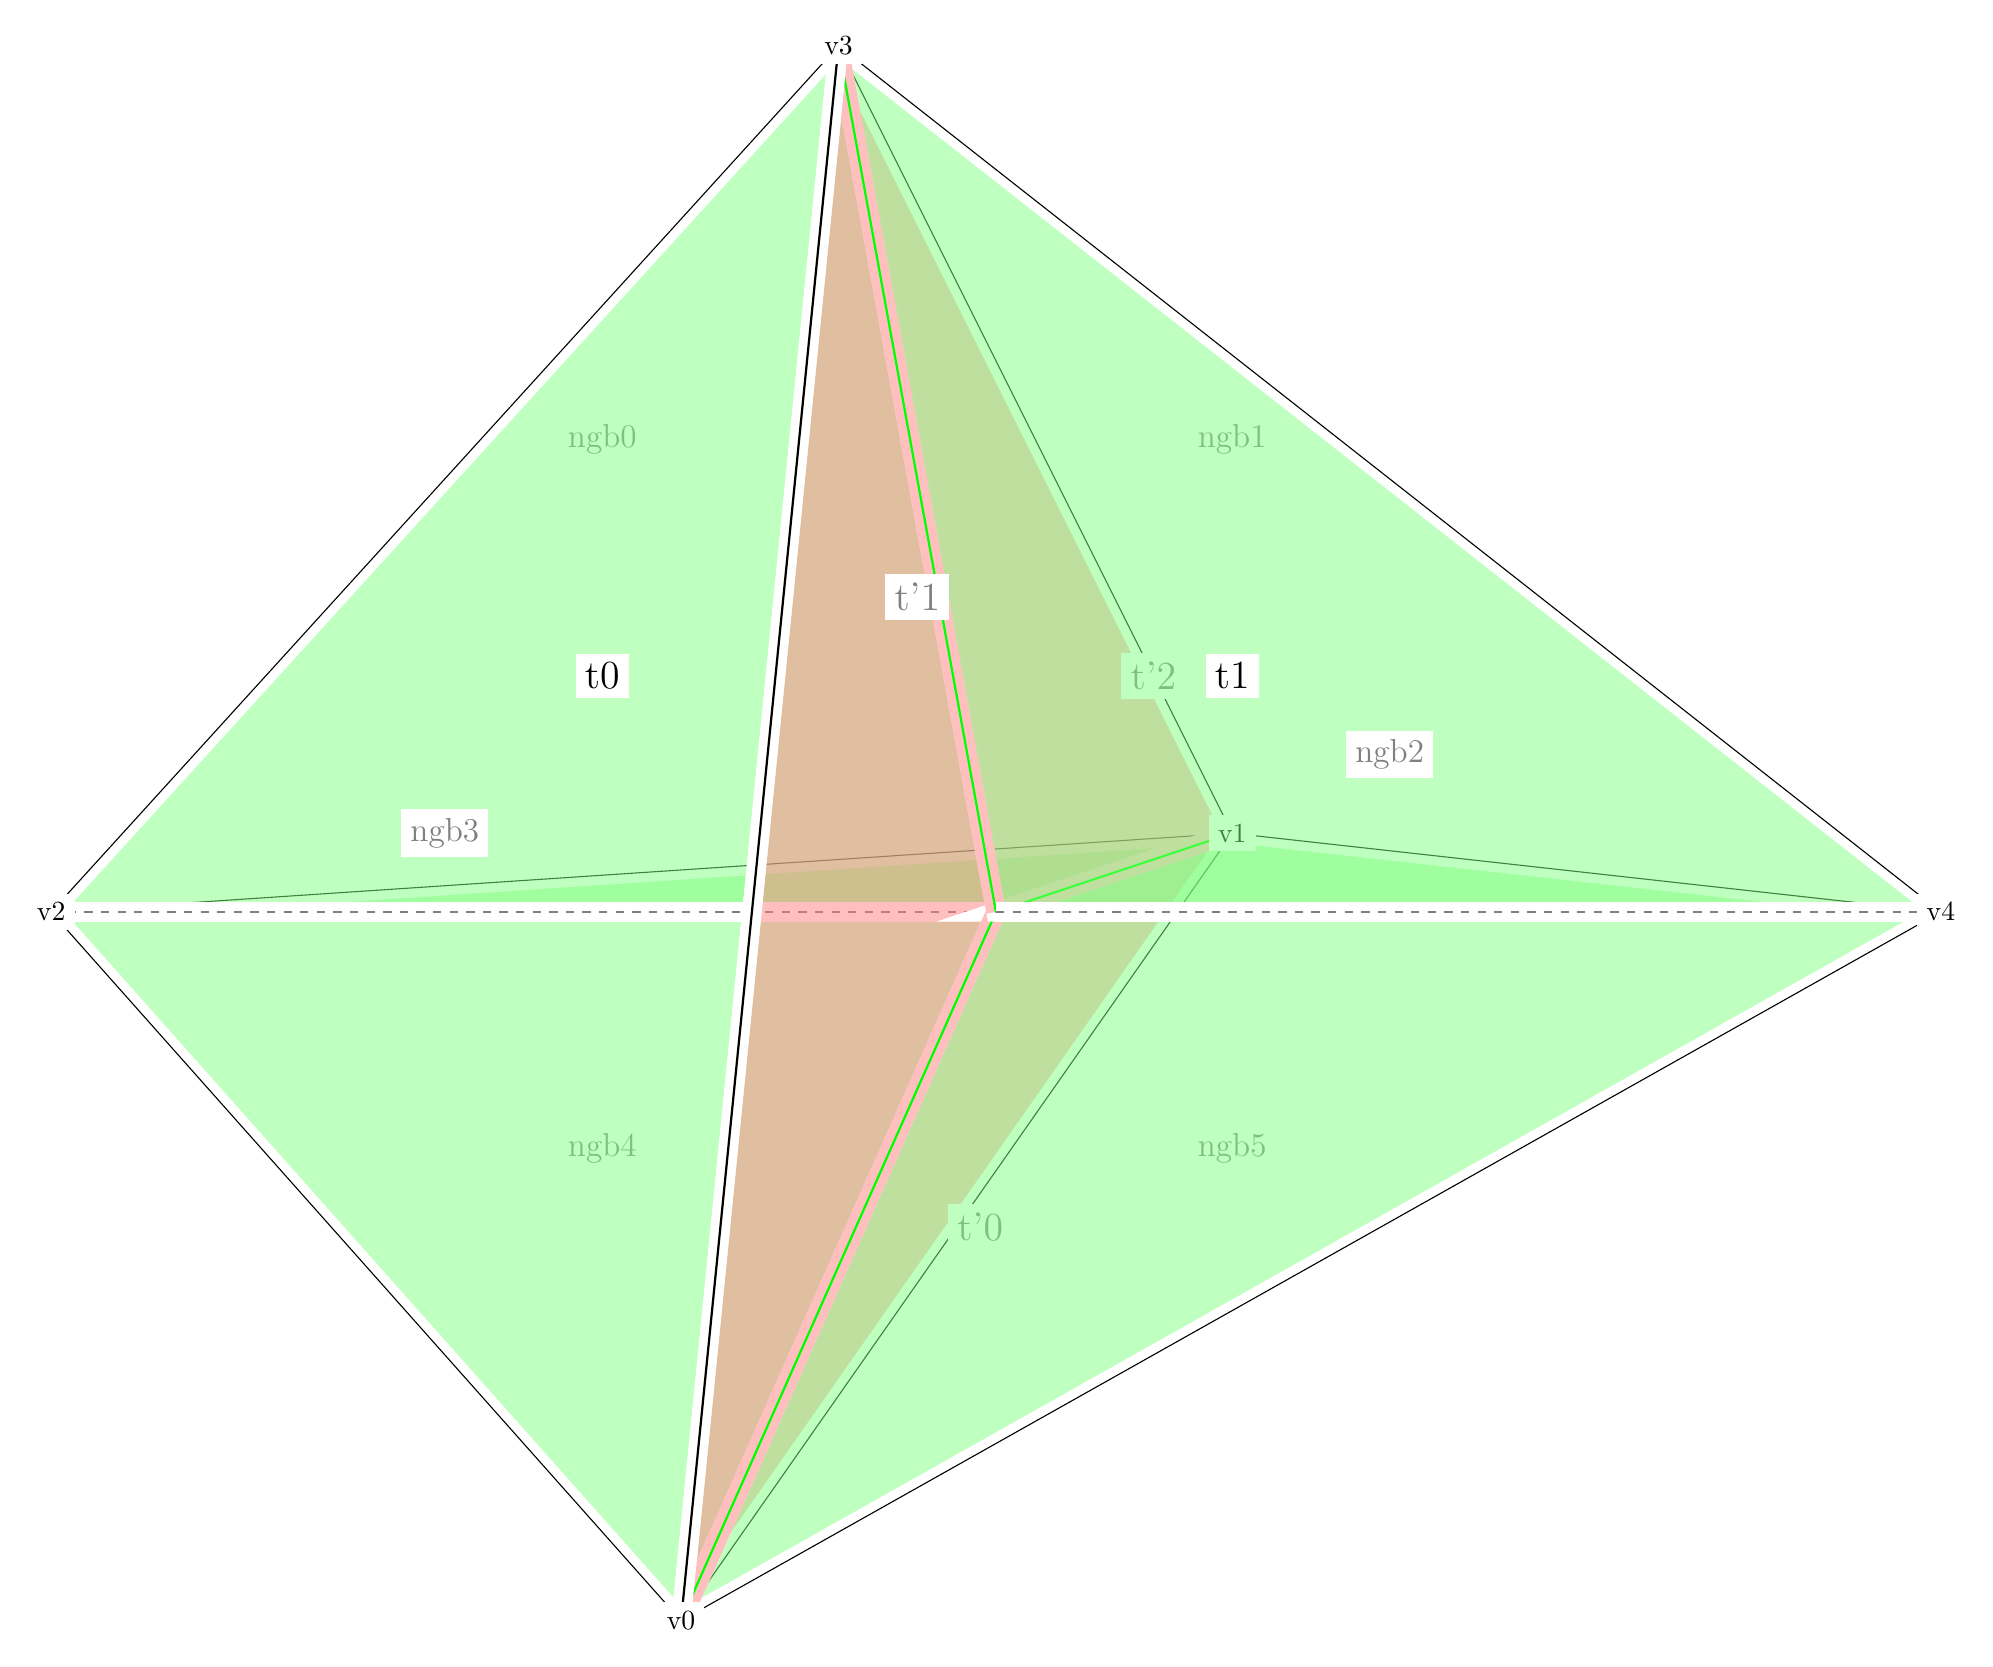
\begin{tikzpicture}[node distance=4.5cm]
\coordinate (c3) at (0.0cm, 0.0cm);
\coordinate (c1) at (5.0cm, -10.0cm);
\coordinate (c2) at (-10.0cm, -11.0cm);
\coordinate (c0) at (-2.0cm, -20.0cm);
\coordinate (c4) at (14.0cm, -11.0cm);
\coordinate (intersect) at (2.0cm, -11.0cm);

\drawLinewithBG{c1}{c3}{arrow}
\drawLinewithBG{c1}{c2}{arrow}
\drawLinewithBG{c0}{c1}{arrow}
\drawLinewithBG{c0}{c2}{arrow}
\drawLinewithBG{c2}{c3}{arrow}

\drawLinewithBG{c0}{c4}{arrow}
\drawLinewithBG{c1}{c4}{arrow}
\drawLinewithBG{c3}{c4}{arrow}

\node [stealthnode, xshift = -3.0cm, yshift = -5.0cm] {\large ngb0};
\node [stealthnode, xshift = 5.0cm, yshift = -5.0cm] {\large ngb1};
\node [stealthnode, xshift = -3.0cm, yshift = -14.0cm] {\large ngb4};
\node [stealthnode, xshift = 5.0cm, yshift = -14.0cm] {\large ngb5};

\drawFace{c1}{c2}{intersect}{green}
\drawFace{c0}{c2}{intersect}{green}
\drawFace{c3}{c2}{intersect}{green}

\drawLinewithBG{c2}{intersect}{stealtharrow}

\drawFace{c0}{c1}{c3}{red}

\node [stealthnode, xshift = 1.8cm, yshift = -15.0cm] {\Large t'0};

\drawFace{c1}{c4}{intersect}{green}
\drawIntersectLine{c1}{intersect}{arrow}{red}{green}
\drawFace{c0}{c4}{intersect}{green}
\drawIntersectLine{c0}{intersect}{arrow}{red}{green}
\node (v1) [node, xshift = 5.0cm, yshift=-10.0cm] {v1};
\node [stealthnode, xshift = 4.0cm, yshift = -8.0cm] {\Large t'2};

\drawFace{c3}{c4}{intersect}{green}
\drawIntersectLine{c3}{intersect}{arrow}{red}{green}

\drawLinewithBG{intersect}{c4}{stealtharrow}

\node [node, xshift = -3.0cm, yshift = -8.0cm] {\Large t0};
\node [node, xshift = 5.0cm, yshift = -8.0cm] {\Large t1};

\drawLinewithBG{c0}{c3}{arrow}

\node [stealthnode, xshift = 1.0cm, yshift = -7.0cm] {\Large t'1};

\node [stealthnode, xshift = 7.0cm, yshift = -9.0cm] {\large ngb2};
\node [stealthnode, xshift = -5.0cm, yshift = -10.0cm] {\large ngb3};

\node (v3) [node] {v3};
\node (v2) [node, xshift = -10.0cm, yshift=-11.0cm] {v2};
\node (v0) [node, xshift = -2.0cm, yshift=-20.0cm] {v0};
\node (v4) [node, xshift = 14.0cm, yshift=-11.0cm] {v4};

\end{tikzpicture}

\end{document}
